% !TeX root = ../main.tex
\chapter{Limitations}\label{chapter:limitations}
This chapter points out the most important limitations and problems during simulation so the solutions to these problems are considered as future works in order to improve the implementation.
\section{sensor measurement and access to a suitable sensor}
As already mentioned above, Carla is a very new simulator which is still under active development. Many of its features are still under test. Among them, we can point to the sensors that are currently offered by Carla. Popular sensor for autonomous parking during recent years was UltraSonic sensors \cite{UltraSonic} but this sensor is not yet presented by Carla. The other choice was Radar sensor which has also provided great results in autonomous driving project during last years \cite{Radar}. However, Carla offers Lidar sensor and use of Lidars for autonomous parking project would be a really novel idea as most of the previous methods were using UltraSonics so by testing this algorithm with Lidar, we could compare the results to Ultrasonic methods. The problem was that the output data we were receiving from Lidar sensor were not totally reliable and perfect, i.e, they did not contain all information of surrounding obstacles and also the 3D visual results(extracted as .ply formats) were not clear enough to make range measurements. Hence, in the limited time of thesis research we were not able to figure out Lidar problems or fix it for our project. Last solution was to substitute Lidar with other sensors offered by Carla. Obstacle sensors and their out put results were the most suitable choice for this work. The idea of this sensor is to detect surrounding obstacles and get the distance to them which was what we were searching for. However, in the earlier version of Carla that we were using, obstacle sensor was not working correctly as the detection of obstacle was a problem in earlier version and finally in Carla version 0.9.5, it has been improved so in the time of publishing this version by Carla developers, we finally could use sensors in our project but still measurement(like distance to detected object) was not working. Fig \ref{fig:obst} shows some results of distance information provided by obstacle sensor. As it has been shown it always shows the same distance. The problem was because of a mistake in the sensor code that it gets Radius measurements instead of distance which we tried to fix this problem and finally get the distance  from it. However, for the parking maneuver to get the parking area measurements and information like lateral displacement of parking bay, distance to other obstacles like side of the parking-bay should be measured so sensor should detect objects other than vehicles like street curbs or sides of the parking place. Instead of getting the distance to the side of the street, distances to the side of the parked vehicles were measured and in this way we just made an estimation of the lateral displacement of the parking-bay which is not an exact measurement. So finding of a perfect sensor which would help us to meet our expectation and measurement goals could be considered as a future work that would also results on better implementation.
\begin{figure}
    \begin{tabular}{c|c}
         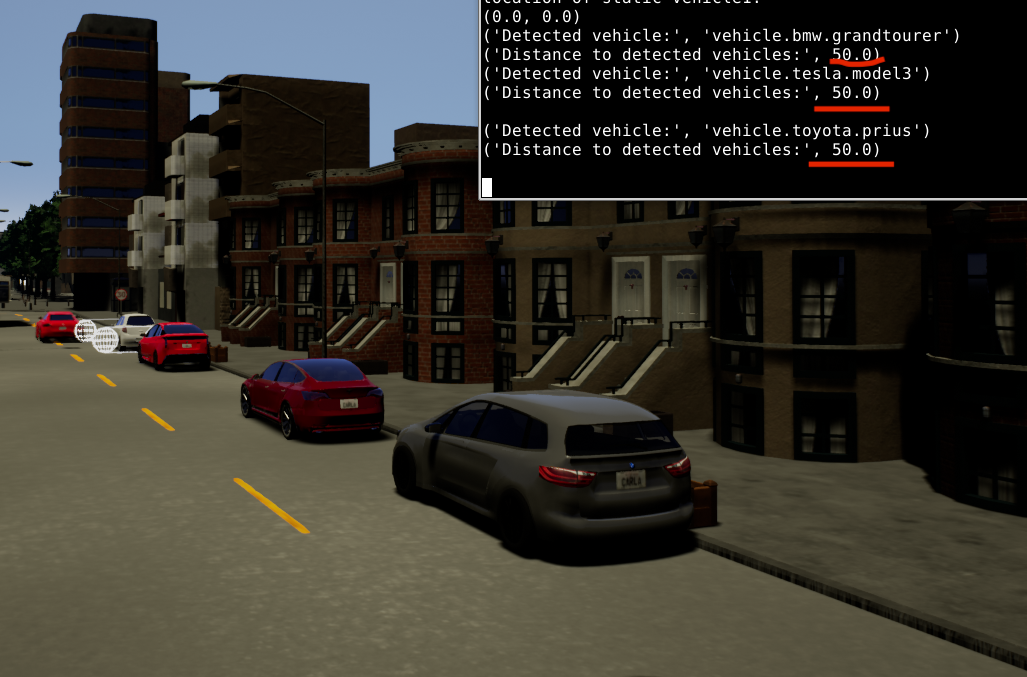
\includegraphics[width=7cm, height=6cm]{images/obst2.png} 
         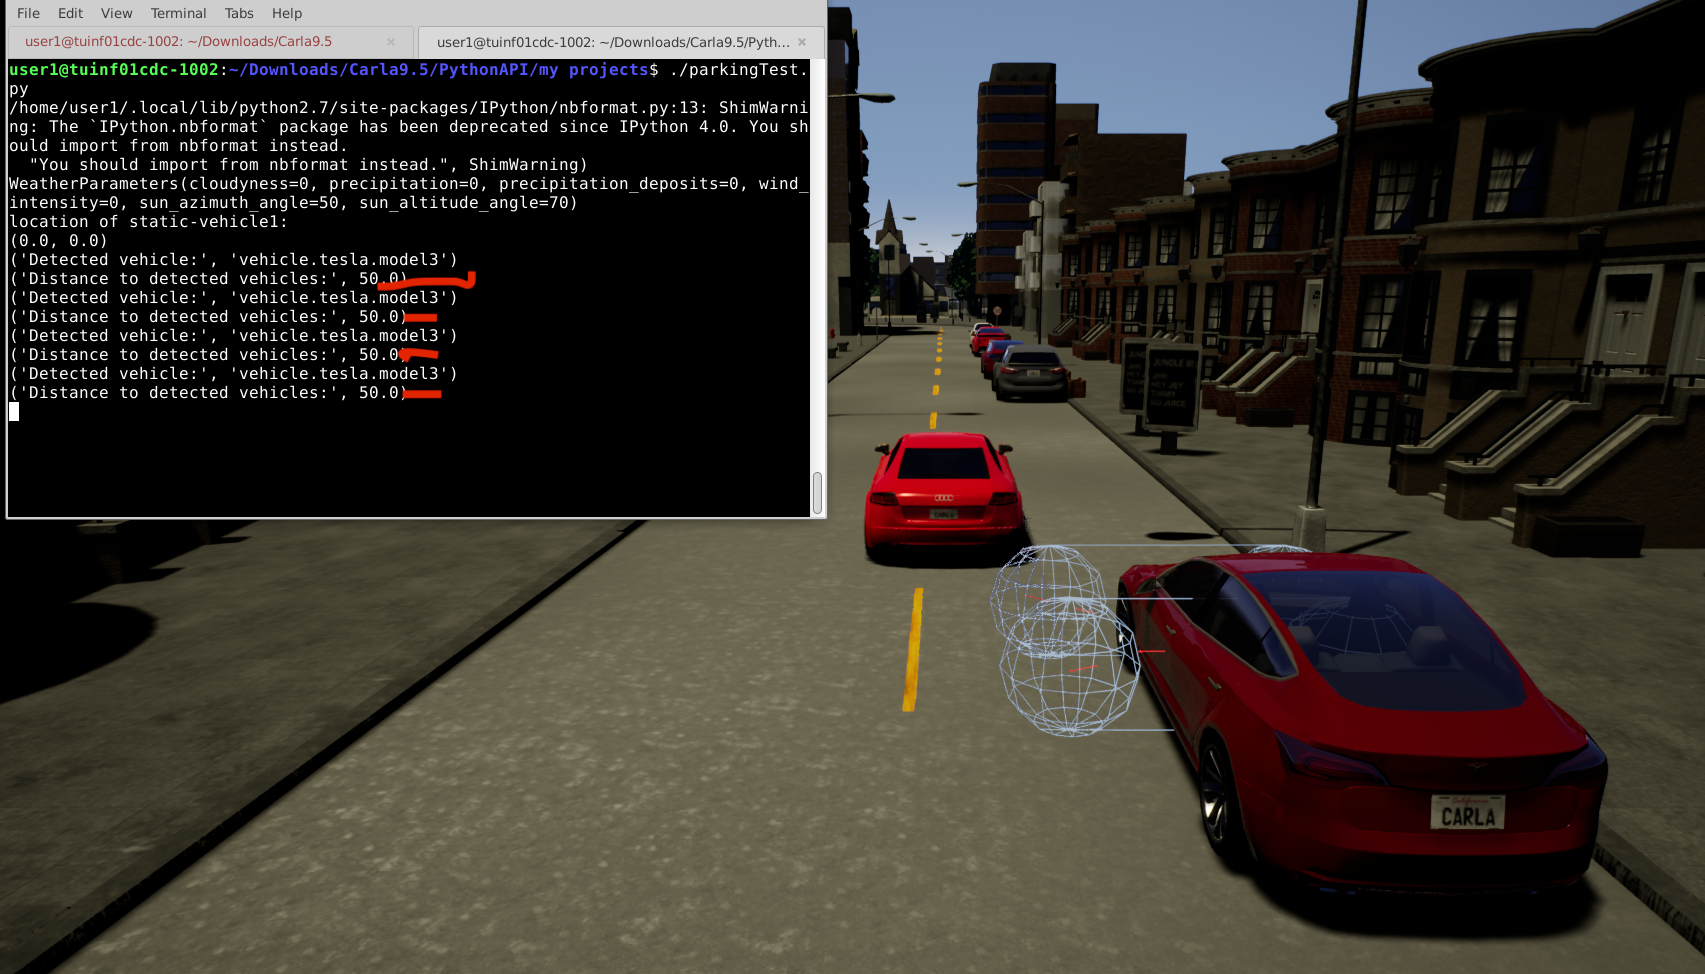
\includegraphics[width=7cm, height=6cm]{images/obst1.png}
    \end{tabular}
    \caption{Obstacle Sensor Results}
    \label{fig:obst}
\end{figure}
\section{API problems}
The main language supported by Carla is Python as its API is PythonAPI but it is also possible to add C++ through libCarla(library provided by Carla). One of the problem as it has already been mentioned in the previous chapters, was using Matlab and its tools for machine learning. Although we managed to make an interface between Matlab and python and finally enjoyed the machine learning tools and libraries of Matlab, this interface made a detection process really slow and we had a synchronization problem between Matlab and python as we decided to make interruption by stopping vehicle and deactivating sensors in each process but this several stop/move vehicle made the program look a bit different from real world where a real driver searching for a parking place and also several connection and disconnection to Matlab engine causes OS problem and when these connect/disconnect are a lot, they stopped simulator from running so the program will be crashed and finally it the whole system and OS will be stopped. These are some of the API limitation during simulation.

